


% Header, overrides base

    % Make sure that the sphinx doc style knows who it inherits from.
    \def\sphinxdocclass{article}

    % Declare the document class
    \documentclass[letterpaper,10pt,english]{/Users/mlhamel/venv/apius/lib/python2.7/site-packages/sphinx/texinputs/sphinxhowto}

    % Imports
    \usepackage[utf8]{inputenc}
    \DeclareUnicodeCharacter{00A0}{\\nobreakspace}
    \usepackage[T1]{fontenc}
    \usepackage{babel}
    \usepackage{times}
    \usepackage{import}
    \usepackage[Bjarne]{/Users/mlhamel/venv/apius/lib/python2.7/site-packages/sphinx/texinputs/fncychap}
    \usepackage{longtable}
    \usepackage{/Users/mlhamel/venv/apius/lib/python2.7/site-packages/sphinx/texinputs/sphinx}
    \usepackage{multirow}

    \usepackage{amsmath}
    \usepackage{amssymb}
    \usepackage{ucs}
    \usepackage{enumerate}

    % Used to make the Input/Output rules follow around the contents.
    \usepackage{needspace}

    % Pygments requirements
    \usepackage{fancyvrb}
    \usepackage{color}
    % ansi colors additions
    \definecolor{darkgreen}{rgb}{.12,.54,.11}
    \definecolor{lightgray}{gray}{.95}
    \definecolor{brown}{rgb}{0.54,0.27,0.07}
    \definecolor{purple}{rgb}{0.5,0.0,0.5}
    \definecolor{darkgray}{gray}{0.25}
    \definecolor{lightred}{rgb}{1.0,0.39,0.28}
    \definecolor{lightgreen}{rgb}{0.48,0.99,0.0}
    \definecolor{lightblue}{rgb}{0.53,0.81,0.92}
    \definecolor{lightpurple}{rgb}{0.87,0.63,0.87}
    \definecolor{lightcyan}{rgb}{0.5,1.0,0.83}

    % Needed to box output/input
    \usepackage{tikz}
        \usetikzlibrary{calc,arrows,shadows}
    \usepackage[framemethod=tikz]{mdframed}

    \usepackage{alltt}

    % Used to load and display graphics
    \usepackage{graphicx}
    \graphicspath{ {figs/} }
    \usepackage[Export]{adjustbox} % To resize

    % used so that images for notebooks which have spaces in the name can still be included
    \usepackage{grffile}


    % For formatting output while also word wrapping.
    \usepackage{listings}
    \lstset{breaklines=true}
    \lstset{basicstyle=\small\ttfamily}
    \def\smaller{\fontsize{9.5pt}{9.5pt}\selectfont}

    %Pygments definitions
    
\makeatletter
\def\PY@reset{\let\PY@it=\relax \let\PY@bf=\relax%
    \let\PY@ul=\relax \let\PY@tc=\relax%
    \let\PY@bc=\relax \let\PY@ff=\relax}
\def\PY@tok#1{\csname PY@tok@#1\endcsname}
\def\PY@toks#1+{\ifx\relax#1\empty\else%
    \PY@tok{#1}\expandafter\PY@toks\fi}
\def\PY@do#1{\PY@bc{\PY@tc{\PY@ul{%
    \PY@it{\PY@bf{\PY@ff{#1}}}}}}}
\def\PY#1#2{\PY@reset\PY@toks#1+\relax+\PY@do{#2}}

\expandafter\def\csname PY@tok@gd\endcsname{\def\PY@tc##1{\textcolor[rgb]{0.63,0.00,0.00}{##1}}}
\expandafter\def\csname PY@tok@gu\endcsname{\let\PY@bf=\textbf\def\PY@tc##1{\textcolor[rgb]{0.50,0.00,0.50}{##1}}}
\expandafter\def\csname PY@tok@gt\endcsname{\def\PY@tc##1{\textcolor[rgb]{0.00,0.27,0.87}{##1}}}
\expandafter\def\csname PY@tok@gs\endcsname{\let\PY@bf=\textbf}
\expandafter\def\csname PY@tok@gr\endcsname{\def\PY@tc##1{\textcolor[rgb]{1.00,0.00,0.00}{##1}}}
\expandafter\def\csname PY@tok@cm\endcsname{\let\PY@it=\textit\def\PY@tc##1{\textcolor[rgb]{0.25,0.50,0.50}{##1}}}
\expandafter\def\csname PY@tok@vg\endcsname{\def\PY@tc##1{\textcolor[rgb]{0.10,0.09,0.49}{##1}}}
\expandafter\def\csname PY@tok@m\endcsname{\def\PY@tc##1{\textcolor[rgb]{0.40,0.40,0.40}{##1}}}
\expandafter\def\csname PY@tok@mh\endcsname{\def\PY@tc##1{\textcolor[rgb]{0.40,0.40,0.40}{##1}}}
\expandafter\def\csname PY@tok@go\endcsname{\def\PY@tc##1{\textcolor[rgb]{0.53,0.53,0.53}{##1}}}
\expandafter\def\csname PY@tok@ge\endcsname{\let\PY@it=\textit}
\expandafter\def\csname PY@tok@vc\endcsname{\def\PY@tc##1{\textcolor[rgb]{0.10,0.09,0.49}{##1}}}
\expandafter\def\csname PY@tok@il\endcsname{\def\PY@tc##1{\textcolor[rgb]{0.40,0.40,0.40}{##1}}}
\expandafter\def\csname PY@tok@cs\endcsname{\let\PY@it=\textit\def\PY@tc##1{\textcolor[rgb]{0.25,0.50,0.50}{##1}}}
\expandafter\def\csname PY@tok@cp\endcsname{\def\PY@tc##1{\textcolor[rgb]{0.74,0.48,0.00}{##1}}}
\expandafter\def\csname PY@tok@gi\endcsname{\def\PY@tc##1{\textcolor[rgb]{0.00,0.63,0.00}{##1}}}
\expandafter\def\csname PY@tok@gh\endcsname{\let\PY@bf=\textbf\def\PY@tc##1{\textcolor[rgb]{0.00,0.00,0.50}{##1}}}
\expandafter\def\csname PY@tok@ni\endcsname{\let\PY@bf=\textbf\def\PY@tc##1{\textcolor[rgb]{0.60,0.60,0.60}{##1}}}
\expandafter\def\csname PY@tok@nl\endcsname{\def\PY@tc##1{\textcolor[rgb]{0.63,0.63,0.00}{##1}}}
\expandafter\def\csname PY@tok@nn\endcsname{\let\PY@bf=\textbf\def\PY@tc##1{\textcolor[rgb]{0.00,0.00,1.00}{##1}}}
\expandafter\def\csname PY@tok@no\endcsname{\def\PY@tc##1{\textcolor[rgb]{0.53,0.00,0.00}{##1}}}
\expandafter\def\csname PY@tok@na\endcsname{\def\PY@tc##1{\textcolor[rgb]{0.49,0.56,0.16}{##1}}}
\expandafter\def\csname PY@tok@nb\endcsname{\def\PY@tc##1{\textcolor[rgb]{0.00,0.50,0.00}{##1}}}
\expandafter\def\csname PY@tok@nc\endcsname{\let\PY@bf=\textbf\def\PY@tc##1{\textcolor[rgb]{0.00,0.00,1.00}{##1}}}
\expandafter\def\csname PY@tok@nd\endcsname{\def\PY@tc##1{\textcolor[rgb]{0.67,0.13,1.00}{##1}}}
\expandafter\def\csname PY@tok@ne\endcsname{\let\PY@bf=\textbf\def\PY@tc##1{\textcolor[rgb]{0.82,0.25,0.23}{##1}}}
\expandafter\def\csname PY@tok@nf\endcsname{\def\PY@tc##1{\textcolor[rgb]{0.00,0.00,1.00}{##1}}}
\expandafter\def\csname PY@tok@si\endcsname{\let\PY@bf=\textbf\def\PY@tc##1{\textcolor[rgb]{0.73,0.40,0.53}{##1}}}
\expandafter\def\csname PY@tok@s2\endcsname{\def\PY@tc##1{\textcolor[rgb]{0.73,0.13,0.13}{##1}}}
\expandafter\def\csname PY@tok@vi\endcsname{\def\PY@tc##1{\textcolor[rgb]{0.10,0.09,0.49}{##1}}}
\expandafter\def\csname PY@tok@nt\endcsname{\let\PY@bf=\textbf\def\PY@tc##1{\textcolor[rgb]{0.00,0.50,0.00}{##1}}}
\expandafter\def\csname PY@tok@nv\endcsname{\def\PY@tc##1{\textcolor[rgb]{0.10,0.09,0.49}{##1}}}
\expandafter\def\csname PY@tok@s1\endcsname{\def\PY@tc##1{\textcolor[rgb]{0.73,0.13,0.13}{##1}}}
\expandafter\def\csname PY@tok@sh\endcsname{\def\PY@tc##1{\textcolor[rgb]{0.73,0.13,0.13}{##1}}}
\expandafter\def\csname PY@tok@sc\endcsname{\def\PY@tc##1{\textcolor[rgb]{0.73,0.13,0.13}{##1}}}
\expandafter\def\csname PY@tok@sx\endcsname{\def\PY@tc##1{\textcolor[rgb]{0.00,0.50,0.00}{##1}}}
\expandafter\def\csname PY@tok@bp\endcsname{\def\PY@tc##1{\textcolor[rgb]{0.00,0.50,0.00}{##1}}}
\expandafter\def\csname PY@tok@c1\endcsname{\let\PY@it=\textit\def\PY@tc##1{\textcolor[rgb]{0.25,0.50,0.50}{##1}}}
\expandafter\def\csname PY@tok@kc\endcsname{\let\PY@bf=\textbf\def\PY@tc##1{\textcolor[rgb]{0.00,0.50,0.00}{##1}}}
\expandafter\def\csname PY@tok@c\endcsname{\let\PY@it=\textit\def\PY@tc##1{\textcolor[rgb]{0.25,0.50,0.50}{##1}}}
\expandafter\def\csname PY@tok@mf\endcsname{\def\PY@tc##1{\textcolor[rgb]{0.40,0.40,0.40}{##1}}}
\expandafter\def\csname PY@tok@err\endcsname{\def\PY@bc##1{\setlength{\fboxsep}{0pt}\fcolorbox[rgb]{1.00,0.00,0.00}{1,1,1}{\strut ##1}}}
\expandafter\def\csname PY@tok@kd\endcsname{\let\PY@bf=\textbf\def\PY@tc##1{\textcolor[rgb]{0.00,0.50,0.00}{##1}}}
\expandafter\def\csname PY@tok@ss\endcsname{\def\PY@tc##1{\textcolor[rgb]{0.10,0.09,0.49}{##1}}}
\expandafter\def\csname PY@tok@sr\endcsname{\def\PY@tc##1{\textcolor[rgb]{0.73,0.40,0.53}{##1}}}
\expandafter\def\csname PY@tok@mo\endcsname{\def\PY@tc##1{\textcolor[rgb]{0.40,0.40,0.40}{##1}}}
\expandafter\def\csname PY@tok@kn\endcsname{\let\PY@bf=\textbf\def\PY@tc##1{\textcolor[rgb]{0.00,0.50,0.00}{##1}}}
\expandafter\def\csname PY@tok@mi\endcsname{\def\PY@tc##1{\textcolor[rgb]{0.40,0.40,0.40}{##1}}}
\expandafter\def\csname PY@tok@gp\endcsname{\let\PY@bf=\textbf\def\PY@tc##1{\textcolor[rgb]{0.00,0.00,0.50}{##1}}}
\expandafter\def\csname PY@tok@o\endcsname{\def\PY@tc##1{\textcolor[rgb]{0.40,0.40,0.40}{##1}}}
\expandafter\def\csname PY@tok@kr\endcsname{\let\PY@bf=\textbf\def\PY@tc##1{\textcolor[rgb]{0.00,0.50,0.00}{##1}}}
\expandafter\def\csname PY@tok@s\endcsname{\def\PY@tc##1{\textcolor[rgb]{0.73,0.13,0.13}{##1}}}
\expandafter\def\csname PY@tok@kp\endcsname{\def\PY@tc##1{\textcolor[rgb]{0.00,0.50,0.00}{##1}}}
\expandafter\def\csname PY@tok@w\endcsname{\def\PY@tc##1{\textcolor[rgb]{0.73,0.73,0.73}{##1}}}
\expandafter\def\csname PY@tok@kt\endcsname{\def\PY@tc##1{\textcolor[rgb]{0.69,0.00,0.25}{##1}}}
\expandafter\def\csname PY@tok@ow\endcsname{\let\PY@bf=\textbf\def\PY@tc##1{\textcolor[rgb]{0.67,0.13,1.00}{##1}}}
\expandafter\def\csname PY@tok@sb\endcsname{\def\PY@tc##1{\textcolor[rgb]{0.73,0.13,0.13}{##1}}}
\expandafter\def\csname PY@tok@k\endcsname{\let\PY@bf=\textbf\def\PY@tc##1{\textcolor[rgb]{0.00,0.50,0.00}{##1}}}
\expandafter\def\csname PY@tok@se\endcsname{\let\PY@bf=\textbf\def\PY@tc##1{\textcolor[rgb]{0.73,0.40,0.13}{##1}}}
\expandafter\def\csname PY@tok@sd\endcsname{\let\PY@it=\textit\def\PY@tc##1{\textcolor[rgb]{0.73,0.13,0.13}{##1}}}

\def\PYZbs{\char`\\}
\def\PYZus{\char`\_}
\def\PYZob{\char`\{}
\def\PYZcb{\char`\}}
\def\PYZca{\char`\^}
\def\PYZam{\char`\&}
\def\PYZlt{\char`\<}
\def\PYZgt{\char`\>}
\def\PYZsh{\char`\#}
\def\PYZpc{\char`\%}
\def\PYZdl{\char`\$}
\def\PYZhy{\char`\-}
\def\PYZsq{\char`\'}
\def\PYZdq{\char`\"}
\def\PYZti{\char`\~}
% for compatibility with earlier versions
\def\PYZat{@}
\def\PYZlb{[}
\def\PYZrb{]}
\makeatother


    %Set pygments styles if needed...
    
        \definecolor{nbframe-border}{rgb}{0.867,0.867,0.867}
        \definecolor{nbframe-bg}{rgb}{0.969,0.969,0.969}
        \definecolor{nbframe-in-prompt}{rgb}{0.0,0.0,0.502}
        \definecolor{nbframe-out-prompt}{rgb}{0.545,0.0,0.0}

        \newenvironment{ColorVerbatim}
        {\begin{mdframed}[%
            roundcorner=1.0pt, %
            backgroundcolor=nbframe-bg, %
            userdefinedwidth=1\linewidth, %
            leftmargin=0.1\linewidth, %
            innerleftmargin=0pt, %
            innerrightmargin=0pt, %
            linecolor=nbframe-border, %
            linewidth=1pt, %
            usetwoside=false, %
            everyline=true, %
            innerlinewidth=3pt, %
            innerlinecolor=nbframe-bg, %
            middlelinewidth=1pt, %
            middlelinecolor=nbframe-bg, %
            outerlinewidth=0.5pt, %
            outerlinecolor=nbframe-border, %
            needspace=0pt
        ]}
        {\end{mdframed}}
        
        \newenvironment{InvisibleVerbatim}
        {\begin{mdframed}[leftmargin=0.1\linewidth,innerleftmargin=3pt,innerrightmargin=3pt, userdefinedwidth=1\linewidth, linewidth=0pt, linecolor=white, usetwoside=false]}
        {\end{mdframed}}

        \renewenvironment{Verbatim}[1][\unskip]
        {\begin{alltt}\smaller}
        {\end{alltt}}
    

    % Help prevent overflowing lines due to urls and other hard-to-break 
    % entities.  This doesn't catch everything...
    \sloppy

    % Document level variables
    \title{apius}
    \date{October 24, 2013}
    \release{}
    \author{Unknown Author}
    \renewcommand{\releasename}{}

    % TODO: Add option for the user to specify a logo for his/her export.
    \newcommand{\sphinxlogo}{}

    % Make the index page of the document.
    \makeindex

    % Import sphinx document type specifics.
     


% Body

    % Start of the document
    \begin{document}

        
            \maketitle
        

        


        
        \part{APIUS.py - L'état du Python }Mathieu Leduc-Hamel

Programmeur Python mais aussi:

 Du haut de ma petite expérience Pythonesque et de ce notebook,
j'aimerais vous faire aimer ce langage\section{L'histoire de Python}\subsection{La définition officielle}\label{la-définition-officielle}

Python est un langage de programmation objet, multi-paradigme et
multi-plateformes. Il favorise la programmation impérative structurée et
orientée objet. Il est doté d'un typage dynamique fort, d'une gestion
automatique de la mémoire par ramasse-miettes et d'un système de gestion
d'exceptions ; il est ainsi similaire à Perl, Ruby, Scheme, Smalltalk et
Tcl.

http://fr.wikipedia.org/wiki/Python\_\%28langage\%29\subsection{Qu'est-ce que ça veut dire
?}\label{quest-ce-que-ça-veut-dire}

Que Python est un language libre, moderne de programmation et qu'il est
écrit \textbf{actuellement} en C (CPython).

    % Make sure that atleast 4 lines are below the HR
    \needspace{4\baselineskip}

    
        \vspace{6pt}
        \makebox[0.1\linewidth]{\smaller\hfill\tt\color{nbframe-in-prompt}In\hspace{4pt}{[}15{]}:\hspace{4pt}}\\*
        \vspace{-2.65\baselineskip}
        \begin{ColorVerbatim}
            \vspace{-0.7\baselineskip}
            \begin{Verbatim}[commandchars=\\\{\}]
\PY{k+kn}{from} \PY{n+nn}{pyquery} \PY{k+kn}{import} \PY{n}{PyQuery} \PY{k}{as} \PY{n}{pq}
\PY{n}{element} \PY{o}{=} \PY{n}{pq}\PY{p}{(}\PY{n}{url}\PY{o}{=}\PY{l+s}{\PYZdq{}}\PY{l+s}{http://www.python.org/2.7/license.html}\PY{l+s}{\PYZdq{}}\PY{p}{)}\PY{o}{.}\PY{n}{find}\PY{p}{(}\PY{l+s}{\PYZdq{}}\PY{l+s}{img}\PY{l+s}{\PYZdq{}}\PY{p}{)}\PY{p}{[}\PY{o}{\PYZhy{}}\PY{l+m+mi}{1}\PY{p}{]}
\PY{n}{Image}\PY{p}{(}\PY{l+s}{\PYZdq{}}\PY{l+s}{http://www.python.org}\PY{l+s}{\PYZdq{}} \PY{o}{+} \PY{n}{element}\PY{o}{.}\PY{n}{attrib}\PY{p}{[}\PY{l+s}{\PYZdq{}}\PY{l+s}{src}\PY{l+s}{\PYZdq{}}\PY{p}{]}\PY{p}{)}
\end{Verbatim}

            
                \vspace{-0.2\baselineskip}
            
        \end{ColorVerbatim}
    

    

        % If the first block is an image, minipage the image.  Else
        % request a certain amount of space for the input text.
        \needspace{4\baselineskip}
        
        

            % Add document contents.
            
                \makebox[0.1\linewidth]{\smaller\hfill\tt\color{nbframe-out-prompt}Out\hspace{4pt}{[}15{]}:\hspace{4pt}}\\*
                \vspace{-2.55\baselineskip}\begin{InvisibleVerbatim}
                \vspace{-0.5\baselineskip}
    \begin{center}
    
\includegraphics[max size={\textwidth}{\textheight}]{apius_files/apius_6_0.png}
    \par
    \end{center}
    
            \end{InvisibleVerbatim}
            
        
    
\subsection{Comment Python évolue}\label{comment-python-évolue}

En soumettant un PEP, comme un blueprints dans le monde d'Ubuntu\subsection{Qu'est-ce qu'un PEP}\label{quest-ce-quun-pep}

\begin{itemize}
\item
  Un PEP c'est un ``Python Enhancement Proposals''
\item
  C'est un document qui sert à proposer des améliorations à Python et à
  sa librairie standard
\item
  Il en existe plus plusieurs centaines, soit:

  \begin{itemize}
  \itemsep1pt\parskip0pt\parsep0pt
  \item
    Meta (des PEPs à propos du processus des PEPs)
  \item
    Autre
  \item
    Accepté
  \item
    Ouvert
  \item
    Terminé
  \item
    Historique
  \item
    Reporté
  \item
    Abandonné
  \end{itemize}
\end{itemize}\subsection{Est-ce que les PEP sont courant
?}\label{est-ce-que-les-pep-sont-courant}

Le plus récent PEP a être accepté l'a été cette semaine, le 22 octobre
2013.

http://www.python.org/dev/peps/pep-0453/

À propos de l'intégration de pip dans la librairie standard, un
installateur de paquets Python.

Bravo à Donald Stufft !\subsection{pep-0020: Le Zen de Python}\label{pep-0020-le-zen-de-python}

C'est ce qui guide le développement de notre language mais aussi notre
travail et notre façon de voir les choses

    % Make sure that atleast 4 lines are below the HR
    \needspace{4\baselineskip}

    
        \vspace{6pt}
        \makebox[0.1\linewidth]{\smaller\hfill\tt\color{nbframe-in-prompt}In\hspace{4pt}{[}4{]}:\hspace{4pt}}\\*
        \vspace{-2.65\baselineskip}
        \begin{ColorVerbatim}
            \vspace{-0.7\baselineskip}
            \begin{Verbatim}[commandchars=\\\{\}]
\PY{k+kn}{from} \PY{n+nn}{pyquery} \PY{k+kn}{import} \PY{n}{PyQuery} \PY{k}{as} \PY{n}{pq}
\PY{k}{print}\PY{p}{(}\PY{n}{pq}\PY{p}{(}\PY{n}{url}\PY{o}{=}\PY{l+s}{\PYZdq{}}\PY{l+s}{http://www.python.org/dev/peps/pep\PYZhy{}0020/}\PY{l+s}{\PYZdq{}}\PY{p}{)}\PY{p}{(}\PY{l+s}{\PYZdq{}}\PY{l+s}{\PYZsh{}body\PYZhy{}main}\PY{l+s}{\PYZdq{}}\PY{p}{)}\PY{o}{.}\PY{n}{find}\PY{p}{(}\PY{l+s}{\PYZdq{}}\PY{l+s}{pre}\PY{l+s}{\PYZdq{}}\PY{p}{)}\PY{p}{[}\PY{l+m+mi}{1}\PY{p}{]}\PY{o}{.}\PY{n}{text}\PY{p}{)}
\end{Verbatim}

            
                \vspace{-0.2\baselineskip}
            
        \end{ColorVerbatim}
    

    

        % If the first block is an image, minipage the image.  Else
        % request a certain amount of space for the input text.
        \needspace{4\baselineskip}
        
        

            % Add document contents.
            
                \begin{InvisibleVerbatim}
                \vspace{-0.5\baselineskip}
\begin{alltt}
    Beautiful is better than ugly.
    Explicit is better than implicit.
    Simple is better than complex.
    Complex is better than complicated.
    Flat is better than nested.
    Sparse is better than dense.
    Readability counts.
    Special cases aren't special enough to break the rules.
    Although practicality beats purity.
    Errors should never pass silently.
    Unless explicitly silenced.
    In the face of ambiguity, refuse the temptation to guess.
    There should be one-- and preferably only one --obvious way to do
it.
    Although that way may not be obvious at first unless you're Dutch.
    Now is better than never.
    Although never is often better than *right* now.
    If the implementation is hard to explain, it's a bad idea.
    If the implementation is easy to explain, it may be a good idea.
    Namespaces are one honking great idea -- let's do more of those!



\end{alltt}

            \end{InvisibleVerbatim}
            
        
    
\subsection{En résumé}\label{en-résumé}

C'est notre code, ça ne fait pas force de lois et on a chacun notre
interpréation du Zen de Python, mais ce qui est clair c'est:

\begin{itemize}
\itemsep1pt\parskip0pt\parsep0pt
\item
  Pragmatisme
\item
  Simplicité
\item
  Éléguance
\item
  Drôle !
\end{itemize}

\begin{quote}
``Python -- This is a Real English Word (honest, look it up!) that
happens to refer to a type of snake, which you'll notice is an object.
With the two vowels, python is quite readable.'' -- Andrew Dalke
\end{quote}

    % Make sure that atleast 4 lines are below the HR
    \needspace{4\baselineskip}

    
        \vspace{6pt}
        \makebox[0.1\linewidth]{\smaller\hfill\tt\color{nbframe-in-prompt}In\hspace{4pt}{[}13{]}:\hspace{4pt}}\\*
        \vspace{-2.65\baselineskip}
        \begin{ColorVerbatim}
            \vspace{-0.7\baselineskip}
            \begin{Verbatim}[commandchars=\\\{\}]
\PY{k+kn}{import} \PY{n+nn}{this}
\end{Verbatim}

            
                \vspace{-0.2\baselineskip}
            
        \end{ColorVerbatim}
    

    

        % If the first block is an image, minipage the image.  Else
        % request a certain amount of space for the input text.
        \needspace{4\baselineskip}
        
        

            % Add document contents.
            
                \begin{InvisibleVerbatim}
                \vspace{-0.5\baselineskip}
\begin{alltt}The Zen of Python, by Tim Peters

Beautiful is better than ugly.
Explicit is better than implicit.
Simple is better than complex.
Complex is better than complicated.
Flat is better than nested.
Sparse is better than dense.
Readability counts.
Special cases aren't special enough to break the rules.
Although practicality beats purity.
Errors should never pass silently.
Unless explicitly silenced.
In the face of ambiguity, refuse the temptation to guess.
There should be one-- and preferably only one --obvious way to do it.
Although that way may not be obvious at first unless you're Dutch.
Now is better than never.
Although never is often better than *right* now.
If the implementation is hard to explain, it's a bad idea.
If the implementation is easy to explain, it may be a good idea.
Namespaces are one honking great idea -- let's do more of those!
\end{alltt}

            \end{InvisibleVerbatim}
            
        
    
\subsection{Guido van Rossum}\label{guido-van-rossum}

    % Make sure that atleast 4 lines are below the HR
    \needspace{4\baselineskip}

    
        \vspace{6pt}
        \makebox[0.1\linewidth]{\smaller\hfill\tt\color{nbframe-in-prompt}In\hspace{4pt}{[}17{]}:\hspace{4pt}}\\*
        \vspace{-2.65\baselineskip}
        \begin{ColorVerbatim}
            \vspace{-0.7\baselineskip}
            \begin{Verbatim}[commandchars=\\\{\}]
\PY{n}{Image}\PY{p}{(}\PY{l+s}{\PYZdq{}}\PY{l+s}{http://pytalent.zandstrasystems.com/Guido\PYZhy{}van\PYZhy{}Rossum\PYZus{}DO6GvRhi.jpg}\PY{l+s}{\PYZdq{}}\PY{p}{)}
\end{Verbatim}

            
                \vspace{-0.2\baselineskip}
            
        \end{ColorVerbatim}
    

    

        % If the first block is an image, minipage the image.  Else
        % request a certain amount of space for the input text.
        \needspace{4\baselineskip}
        
        

            % Add document contents.
            
                \makebox[0.1\linewidth]{\smaller\hfill\tt\color{nbframe-out-prompt}Out\hspace{4pt}{[}17{]}:\hspace{4pt}}\\*
                \vspace{-2.55\baselineskip}\begin{InvisibleVerbatim}
                \vspace{-0.5\baselineskip}
    \begin{center}
    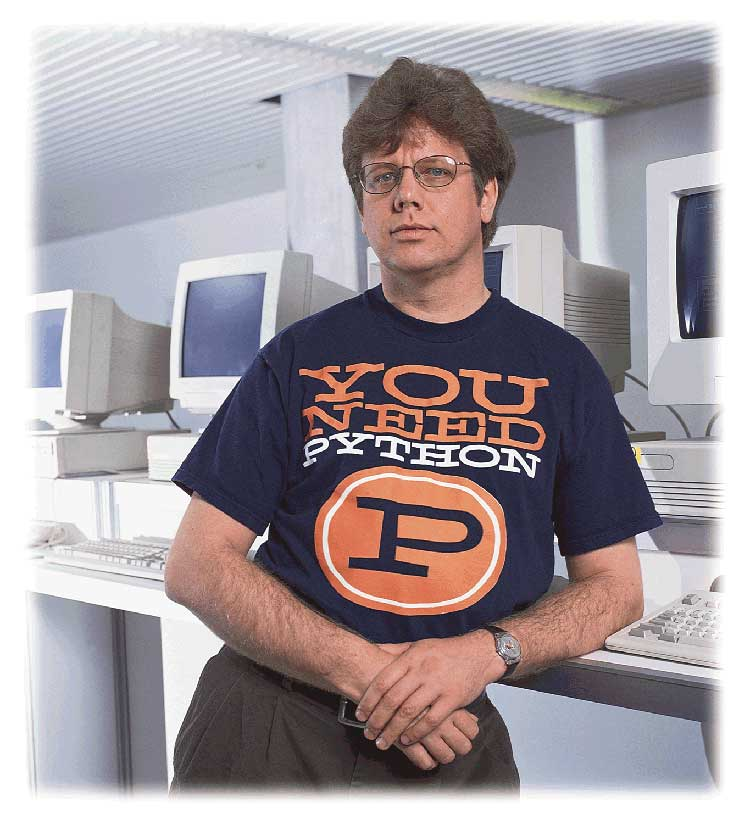
\includegraphics[max size={\textwidth}{\textheight}]{apius_files/apius_15_0.jpeg}
    \par
    \end{center}
    
            \end{InvisibleVerbatim}
            
        
    
\subsection{Qui Guido ?}\label{qui-guido}

\begin{itemize}
\item
  Née aux Pays-Bas, en 1957
\item
  Complété un master en mathématiques en sciences informatiques à
  l'université d'Amsterdam
\item
  Soumet au ministère de la défense américaine une proposition d'un
  nouveau language de programmation en 1999 (Python\ldots{})
\item
  Possède le titre de dictateur bien aimé et à vie (BDFL)
\item
  Travail chez Dropbox depuis Janvier 2013.
\item
  A travaillé dans le passé chez:

  \begin{itemize}
  \itemsep1pt\parskip0pt\parsep0pt
  \item
    Google
  \item
    Elemental Security
  \item
    Zope Corporation
  \item
    BeOpen.com
  \item
    CNRI (où il a créé Python)
  \item
    CWI
  \item
    SARA
  \end{itemize}
\end{itemize}\subsection{L'âge préhistorique}\label{lâge-préhistorique}

\begin{verbatim}
La première version publique de Python date de 1991.

À l'époque Guido était fortement influencé par le LISP et la programmation fonctionnelle.

0.9.0 - Février 1991 

Première publication officielle sur alt.sources.

Python 1.0 - Janvier 1994

Guido travail au CNRI, Corporation for National Research Initiatives 
    
  * Ajout du lambda, map, filter et du reduce.
  
\end{verbatim}\subsection{Les temps modernes}\label{les-temps-modernes}

\begin{verbatim}
Python 2.0 - Octobre 16, 2000

* Ajout des listes par compréhension et du "garbage collector" 

    Python 2.1 - Avril 17, 2001
    
    * Naissance de la PSF
    
    Python 2.2 - Décembre 21, 2001
    
    * Le langage évolue et rafine avec les "nested scope" (la portée des variables)
    
    Python 2.3 - Juillet 29, 2003
    
    * On gagne de la vitesse et on peut le savoir grâce à timeit !
    
    Python 2.4 - Novembre 30, 2004
    
    * Set fait son entrée 
    * Générateurs (pep 289)
    * Décorateurs
    
    Python 2.6 - Octobre 1, 2008
    
    * On structure l'évolution des releases (pep 361) jusqu'à 3.0
    * with et les context managers
    * multiprocessing
    
    Python 2.7 - Juillet 3, 2010
    
    * On backport des modules de Python 3.1
    * Une release de transition
    
\end{verbatim}\subsection{La période contemporaine}\label{la-période-contemporaine}

\begin{verbatim}
Python 3.0 - Décembre 3, 2008

    Python 3.1 - Juin 27, 2009
    
    Python 3.2 - Février 20, 2011
    
    Python 3.3 - Septembre 29, 2012
\end{verbatim}\subsection{Pourquoi migrer à Python
3}\label{pourquoi-migrer-à-python-3}

Selon ``Nick Coghlan's Python Notes''
http://python-notes.boredomandlaziness.org/en/latest/python3/

\begin{itemize}
\itemsep1pt\parskip0pt\parsep0pt
\item
  Supprimer les fonctionalités déjà ``dépréciées''
\item
  Réduire le nombre de mot réservés dans le langage
\item
  Utiliser des conteneur plus efficace en mémoire
\item
  Rendre la librairie standard plus \textbf{PEP8}
\end{itemize}

et\ldots{}\section{Unicode !!!}

    % Make sure that atleast 4 lines are below the HR
    \needspace{4\baselineskip}

    
        \vspace{6pt}
        \makebox[0.1\linewidth]{\smaller\hfill\tt\color{nbframe-in-prompt}In\hspace{4pt}{[}16{]}:\hspace{4pt}}\\*
        \vspace{-2.65\baselineskip}
        \begin{ColorVerbatim}
            \vspace{-0.7\baselineskip}
            \begin{Verbatim}[commandchars=\\\{\}]
\PY{l+s}{\PYZdq{}}\PY{l+s}{évoluton du language}\PY{l+s}{\PYZdq{}}
\end{Verbatim}

            
                \vspace{-0.2\baselineskip}
            
        \end{ColorVerbatim}
    

    

        % If the first block is an image, minipage the image.  Else
        % request a certain amount of space for the input text.
        \needspace{4\baselineskip}
        
        

            % Add document contents.
            
                \makebox[0.1\linewidth]{\smaller\hfill\tt\color{nbframe-out-prompt}Out\hspace{4pt}{[}16{]}:\hspace{4pt}}\\*
                \vspace{-2.55\baselineskip}\begin{InvisibleVerbatim}
                \vspace{-0.5\baselineskip}
\begin{alltt}'\textbackslash{}xc3\textbackslash{}xa9voluton du language'\end{alltt}

            \end{InvisibleVerbatim}
            
        
    
\subsection{Comment va le passage à Python
3}\label{comment-va-le-passage-à-python-3}

\begin{itemize}
\itemsep1pt\parskip0pt\parsep0pt
\item
  Souffrant dans le passé, ça avance bien.
\item
  Porter son code c'est facile (2to3).
\item
  Plupart des packages important ont fait le saut.
\end{itemize}

    % Make sure that atleast 4 lines are below the HR
    \needspace{4\baselineskip}

    
        \vspace{6pt}
        \makebox[0.1\linewidth]{\smaller\hfill\tt\color{nbframe-in-prompt}In\hspace{4pt}{[}29{]}:\hspace{4pt}}\\*
        \vspace{-2.65\baselineskip}
        \begin{ColorVerbatim}
            \vspace{-0.7\baselineskip}
            \begin{Verbatim}[commandchars=\\\{\}]
\PY{k+kn}{from} \PY{n+nn}{IPython.core.display} \PY{k+kn}{import} \PY{n}{HTML}

\PY{n}{HTML}\PY{p}{(}\PY{l+s}{\PYZdq{}}\PY{l+s}{\PYZlt{}iframe src=}\PY{l+s}{\PYZsq{}}\PY{l+s}{https://python3wos.appspot.com/}\PY{l+s}{\PYZsq{}}\PY{l+s}{ height=}\PY{l+s}{\PYZsq{}}\PY{l+s}{600}\PY{l+s}{\PYZsq{}}\PY{l+s}{\PYZgt{}\PYZlt{}/iframe\PYZgt{}}\PY{l+s}{\PYZdq{}}\PY{p}{)}
\end{Verbatim}

            
                \vspace{-0.2\baselineskip}
            
        \end{ColorVerbatim}
    

    

        % If the first block is an image, minipage the image.  Else
        % request a certain amount of space for the input text.
        \needspace{4\baselineskip}
        
        

            % Add document contents.
            
                \makebox[0.1\linewidth]{\smaller\hfill\tt\color{nbframe-out-prompt}Out\hspace{4pt}{[}29{]}:\hspace{4pt}}\\*
                \vspace{-2.55\baselineskip}\begin{InvisibleVerbatim}
                \vspace{-0.5\baselineskip}
\begin{alltt}<IPython.core.display.HTML at 0x10e20c150>\end{alltt}

            \end{InvisibleVerbatim}
            
        
    
\subsection{Évolution de la taille de librairie
standard}\label{évolution-de-la-taille-de-librairie-standard}

    % Make sure that atleast 4 lines are below the HR
    \needspace{4\baselineskip}

    
        \vspace{6pt}
        \makebox[0.1\linewidth]{\smaller\hfill\tt\color{nbframe-in-prompt}In\hspace{4pt}{[}6{]}:\hspace{4pt}}\\*
        \vspace{-2.65\baselineskip}
        \begin{ColorVerbatim}
            \vspace{-0.7\baselineskip}
            \begin{Verbatim}[commandchars=\\\{\}]
\PY{k+kn}{from} \PY{n+nn}{pyquery} \PY{k+kn}{import} \PY{n}{PyQuery} \PY{k}{as} \PY{n}{pq}

\PY{n}{base\PYZus{}url} \PY{o}{=} \PY{l+s}{\PYZdq{}}\PY{l+s}{http://docs.python.org/release/}\PY{l+s+si}{\PYZpc{}s}\PY{l+s}{/modindex.html}\PY{l+s}{\PYZdq{}}
\PY{n}{new\PYZus{}url} \PY{o}{=} \PY{l+s}{\PYZdq{}}\PY{l+s}{http://docs.python.org/release/}\PY{l+s+si}{\PYZpc{}s}\PY{l+s}{/py\PYZhy{}modindex.html}\PY{l+s}{\PYZdq{}}
\PY{n}{newer\PYZus{}url} \PY{o}{=} \PY{l+s}{\PYZdq{}}\PY{l+s}{http://docs.python.org/}\PY{l+s+si}{\PYZpc{}s}\PY{l+s}{/py\PYZhy{}modindex.html}\PY{l+s}{\PYZdq{}}

\PY{n}{data} \PY{o}{=} \PY{p}{\PYZob{}}\PY{p}{\PYZcb{}}

\PY{k}{def} \PY{n+nf}{count\PYZus{}modules}\PY{p}{(}\PY{n}{version}\PY{p}{,} \PY{n}{dt}\PY{o}{=}\PY{n+nb+bp}{False}\PY{p}{,} \PY{n}{old}\PY{o}{=}\PY{n+nb+bp}{True}\PY{p}{,} \PY{n}{newer}\PY{o}{=}\PY{n+nb+bp}{False}\PY{p}{)}\PY{p}{:}
    \PY{k}{if} \PY{n}{dt}\PY{p}{:}
        \PY{n}{data}\PY{p}{[}\PY{n}{version}\PY{p}{]} \PY{o}{=} \PY{n+nb}{len}\PY{p}{(}\PY{n}{pq}\PY{p}{(}\PY{n}{url}\PY{o}{=}\PY{n}{base\PYZus{}url} \PY{o}{\PYZpc{}} \PY{n}{version}\PY{p}{)}\PY{o}{.}\PY{n}{find}\PY{p}{(}\PY{l+s}{\PYZdq{}}\PY{l+s}{table dt}\PY{l+s}{\PYZdq{}}\PY{p}{)}\PY{p}{)}     
    \PY{k}{elif} \PY{n}{old}\PY{p}{:}
        \PY{n}{data}\PY{p}{[}\PY{n}{version}\PY{p}{]} \PY{o}{=} \PY{n+nb}{len}\PY{p}{(}\PY{n}{pq}\PY{p}{(}\PY{n}{url}\PY{o}{=}\PY{n}{base\PYZus{}url} \PY{o}{\PYZpc{}} \PY{n}{version}\PY{p}{)}\PY{o}{.}\PY{n}{find}\PY{p}{(}\PY{l+s}{\PYZdq{}}\PY{l+s}{table tt}\PY{l+s}{\PYZdq{}}\PY{p}{)}\PY{p}{)}
    \PY{k}{elif} \PY{n}{newer}\PY{p}{:}
        \PY{n}{data}\PY{p}{[}\PY{n}{version}\PY{p}{]} \PY{o}{=} \PY{n+nb}{len}\PY{p}{(}\PY{n}{pq}\PY{p}{(}\PY{n}{url}\PY{o}{=}\PY{n}{newer\PYZus{}url} \PY{o}{\PYZpc{}} \PY{n}{version}\PY{p}{)}\PY{o}{.}\PY{n}{find}\PY{p}{(}\PY{l+s}{\PYZdq{}}\PY{l+s}{table tt}\PY{l+s}{\PYZdq{}}\PY{p}{)}\PY{p}{)}
    \PY{k}{else}\PY{p}{:}
        \PY{n}{data}\PY{p}{[}\PY{n}{version}\PY{p}{]} \PY{o}{=} \PY{n+nb}{len}\PY{p}{(}\PY{n}{pq}\PY{p}{(}\PY{n}{url}\PY{o}{=}\PY{n}{new\PYZus{}url} \PY{o}{\PYZpc{}} \PY{n}{version}\PY{p}{)}\PY{o}{.}\PY{n}{find}\PY{p}{(}\PY{l+s}{\PYZdq{}}\PY{l+s}{table tt}\PY{l+s}{\PYZdq{}}\PY{p}{)}\PY{p}{)}
    \PY{k}{return} \PY{n}{data}

\PY{k}{for} \PY{n}{v} \PY{o+ow}{in} \PY{n+nb}{range}\PY{p}{(}\PY{l+m+mi}{1}\PY{p}{,} \PY{l+m+mi}{6}\PY{p}{)}\PY{p}{:}
    \PY{n}{count\PYZus{}modules}\PY{p}{(}\PY{l+s}{\PYZdq{}}\PY{l+s}{2.}\PY{l+s+si}{\PYZpc{}d}\PY{l+s}{\PYZdq{}} \PY{o}{\PYZpc{}} \PY{n}{v}\PY{p}{,} \PY{n}{dt}\PY{o}{=}\PY{n+nb+bp}{True}\PY{p}{)}
    
\PY{n}{count\PYZus{}modules}\PY{p}{(}\PY{l+s}{\PYZdq{}}\PY{l+s}{2.6}\PY{l+s}{\PYZdq{}}\PY{p}{)}
\PY{n}{count\PYZus{}modules}\PY{p}{(}\PY{l+s}{\PYZdq{}}\PY{l+s}{2.7}\PY{l+s}{\PYZdq{}}\PY{p}{)}
\PY{n}{count\PYZus{}modules}\PY{p}{(}\PY{l+s}{\PYZdq{}}\PY{l+s}{3.0}\PY{l+s}{\PYZdq{}}\PY{p}{)}
\PY{n}{count\PYZus{}modules}\PY{p}{(}\PY{l+s}{\PYZdq{}}\PY{l+s}{3.1}\PY{l+s}{\PYZdq{}}\PY{p}{)}
\PY{n}{count\PYZus{}modules}\PY{p}{(}\PY{l+s}{\PYZdq{}}\PY{l+s}{3.2}\PY{l+s}{\PYZdq{}}\PY{p}{,} \PY{n}{old}\PY{o}{=}\PY{n+nb+bp}{False}\PY{p}{)}
\PY{k}{print}\PY{p}{(}\PY{n}{count\PYZus{}modules}\PY{p}{(}\PY{l+s}{\PYZdq{}}\PY{l+s}{3.3}\PY{l+s}{\PYZdq{}}\PY{p}{,} \PY{n}{old}\PY{o}{=}\PY{n+nb+bp}{False}\PY{p}{,} \PY{n}{newer}\PY{o}{=}\PY{n+nb+bp}{True}\PY{p}{)}\PY{p}{)}
\end{Verbatim}

            
                \vspace{-0.2\baselineskip}
            
        \end{ColorVerbatim}
    

    

        % If the first block is an image, minipage the image.  Else
        % request a certain amount of space for the input text.
        \needspace{4\baselineskip}
        
        

            % Add document contents.
            
                \begin{InvisibleVerbatim}
                \vspace{-0.5\baselineskip}
\begin{alltt}\{'3.2': 306, '3.3': 313, '3.0': 292, '3.1': 298, '2.3': 314, '2.2':
285, '2.1': 255, '2.7': 430, '2.6': 392, '2.5': 379, '2.4': 362\}
\end{alltt}

            \end{InvisibleVerbatim}
            
        
    
\subsection{Concrètement ça donne ? (merci
matplotlib)}\label{concrètement-ça-donne-merci-matplotlib}

    % Make sure that atleast 4 lines are below the HR
    \needspace{4\baselineskip}

    
        \vspace{6pt}
        \makebox[0.1\linewidth]{\smaller\hfill\tt\color{nbframe-in-prompt}In\hspace{4pt}{[}14{]}:\hspace{4pt}}\\*
        \vspace{-2.65\baselineskip}
        \begin{ColorVerbatim}
            \vspace{-0.7\baselineskip}
            \begin{Verbatim}[commandchars=\\\{\}]
\PY{o}{\PYZpc{}}\PY{k}{pylab} \PY{n}{inline} \PY{o}{\PYZhy{}}\PY{o}{\PYZhy{}}\PY{n}{no}\PY{o}{\PYZhy{}}\PY{n}{import}\PY{o}{\PYZhy{}}\PY{n+nb}{all}

\PY{k+kn}{from} \PY{n+nn}{pylab} \PY{k+kn}{import} \PY{n}{figure}\PY{p}{,} \PY{n}{plot}\PY{p}{,} \PY{n}{title}\PY{p}{,} \PY{n}{xlabel}\PY{p}{,} \PY{n}{ylabel}\PY{p}{,} \PY{n}{show}

\PY{n}{x} \PY{o}{=} \PY{n}{data}\PY{o}{.}\PY{n}{keys}\PY{p}{(}\PY{p}{)}
\PY{n}{x}\PY{o}{.}\PY{n}{sort}\PY{p}{(}\PY{p}{)}
\PY{n}{y} \PY{o}{=} \PY{p}{[}\PY{n}{data}\PY{p}{[}\PY{n}{k}\PY{p}{]} \PY{k}{for} \PY{n}{k} \PY{o+ow}{in} \PY{n}{x}\PY{p}{]}

\PY{n}{figure}\PY{p}{(}\PY{p}{)}
\PY{n}{plot}\PY{p}{(}\PY{n}{x}\PY{p}{,} \PY{n}{y}\PY{p}{,} \PY{l+s}{\PYZsq{}}\PY{l+s}{r}\PY{l+s}{\PYZsq{}}\PY{p}{)}
\PY{n}{xlabel}\PY{p}{(}\PY{l+s}{\PYZsq{}}\PY{l+s}{Version de Python}\PY{l+s}{\PYZsq{}}\PY{p}{)}
\PY{n}{ylabel}\PY{p}{(}\PY{l+s}{\PYZsq{}}\PY{l+s}{Nombre de modules}\PY{l+s}{\PYZsq{}}\PY{p}{)}
\PY{n}{title}\PY{p}{(}\PY{l+s}{u\PYZsq{}}\PY{l+s}{Évolution du nombre de modules dans les STD Python}\PY{l+s}{\PYZsq{}}\PY{p}{)}
\PY{n}{show}\PY{p}{(}\PY{p}{)}
\end{Verbatim}

            
                \vspace{-0.2\baselineskip}
            
        \end{ColorVerbatim}
    

    

        % If the first block is an image, minipage the image.  Else
        % request a certain amount of space for the input text.
        \needspace{4\baselineskip}
        
        

            % Add document contents.
            
                \begin{InvisibleVerbatim}
                \vspace{-0.5\baselineskip}
\begin{alltt}Populating the interactive namespace from numpy and matplotlib
\end{alltt}

            \end{InvisibleVerbatim}
            
                \begin{InvisibleVerbatim}
                \vspace{-0.5\baselineskip}
    \begin{center}
    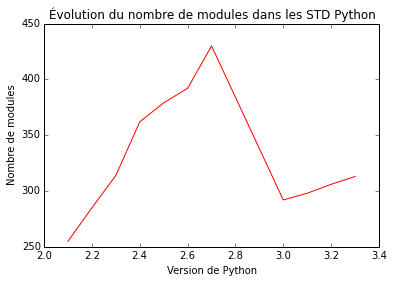
\includegraphics[max size={\textwidth}{\textheight}]{apius_files/apius_28_1.png}
    \par
    \end{center}
    
            \end{InvisibleVerbatim}
            
        
    
\subsection{La post-histoire}\label{la-post-histoire}

\begin{verbatim}
PyPY 1.0 - Juin 2007   

Une complète ré-écriture de Python en Python. Le but de l'opération :

* implanter un compilateur Just-In-time (JIT)
* conserver la compabilité avec le CPython tradionnel
* créer une plateforme d'expérimentation pour les languages de programmation dynamiques

    PyPY 1.2 - Mars 2010
    
    PyPy 1.5 - Avril 2011
    
    PyPy 1.9 - Mars 2012
    
    PyPy 2.1 - Auoût 2013
\end{verbatim}\section{La Communauté}

    % Make sure that atleast 4 lines are below the HR
    \needspace{4\baselineskip}

    
        \vspace{6pt}
        \makebox[0.1\linewidth]{\smaller\hfill\tt\color{nbframe-in-prompt}In\hspace{4pt}{[}35{]}:\hspace{4pt}}\\*
        \vspace{-2.65\baselineskip}
        \begin{ColorVerbatim}
            \vspace{-0.7\baselineskip}
            \begin{Verbatim}[commandchars=\\\{\}]
\PY{k+kn}{from} \PY{n+nn}{IPython.core.display} \PY{k+kn}{import} \PY{n}{Image}
\PY{k+kn}{import} \PY{n+nn}{antigravity}
\PY{n}{Image}\PY{p}{(}\PY{l+s}{\PYZdq{}}\PY{l+s}{http://imgs.xkcd.com/comics/python.png}\PY{l+s}{\PYZdq{}}\PY{p}{)}
\end{Verbatim}

            
                \vspace{-0.2\baselineskip}
            
        \end{ColorVerbatim}
    

    

        % If the first block is an image, minipage the image.  Else
        % request a certain amount of space for the input text.
        \needspace{4\baselineskip}
        
        

            % Add document contents.
            
                \makebox[0.1\linewidth]{\smaller\hfill\tt\color{nbframe-out-prompt}Out\hspace{4pt}{[}35{]}:\hspace{4pt}}\\*
                \vspace{-2.55\baselineskip}\begin{InvisibleVerbatim}
                \vspace{-0.5\baselineskip}
    \begin{center}
    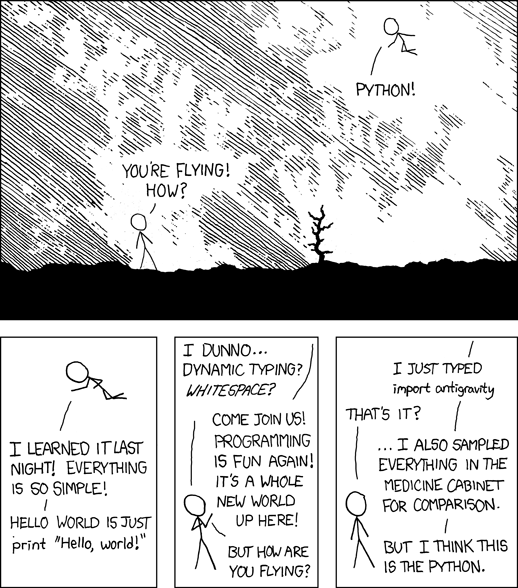
\includegraphics[max size={\textwidth}{\textheight}]{apius_files/apius_31_0.png}
    \par
    \end{center}
    
            \end{InvisibleVerbatim}
            
        
    
\subsection{La Python Software
Foundation}\label{la-python-software-foundation}

\begin{itemize}
\itemsep1pt\parskip0pt\parsep0pt
\item
  Une organization sans but lucratif enregistrée
\item
  Défend et gère le nom de marque Python (Bataille juridique plus tôt
  cette année)
\item
  Aide la formation de nouveaux groupes d'usagers
\item
  Finance le développement de projets Python
\item
  Promouvoit le Python par PyCon
\end{itemize}\subsection{Les groupes d'usagers}\label{les-groupes-dusagers}

\begin{itemize}
\itemsep1pt\parskip0pt\parsep0pt
\item
  Base de la communauté Python
\item
  Des groupe d'usagers sur 5 continents
  (https://wiki.python.org/moin/LocalUserGroups)
\item
  Dans la plupart des langues du monde
\end{itemize}

    % Make sure that atleast 4 lines are below the HR
    \needspace{4\baselineskip}

    
        \vspace{6pt}
        \makebox[0.1\linewidth]{\smaller\hfill\tt\color{nbframe-in-prompt}In\hspace{4pt}{[}5{]}:\hspace{4pt}}\\*
        \vspace{-2.65\baselineskip}
        \begin{ColorVerbatim}
            \vspace{-0.7\baselineskip}
            \begin{Verbatim}[commandchars=\\\{\}]
\PY{k+kn}{from} \PY{n+nn}{pyquery} \PY{k+kn}{import} \PY{n}{PyQuery} \PY{k}{as} \PY{n}{pq}
\PY{n+nb}{len}\PY{p}{(}\PY{n}{pq}\PY{p}{(}\PY{n}{url}\PY{o}{=}\PY{l+s}{\PYZdq{}}\PY{l+s}{https://wiki.python.org/moin/LocalUserGroups}\PY{l+s}{\PYZdq{}}\PY{p}{)}\PY{o}{.}\PY{n}{find}\PY{p}{(}\PY{l+s}{\PYZdq{}}\PY{l+s}{.table\PYZhy{}of\PYZhy{}contents li}\PY{l+s}{\PYZdq{}}\PY{p}{)}\PY{p}{)} \PY{o}{\PYZhy{}} \PY{l+m+mi}{5}
\end{Verbatim}

            
                \vspace{-0.2\baselineskip}
            
        \end{ColorVerbatim}
    

    

        % If the first block is an image, minipage the image.  Else
        % request a certain amount of space for the input text.
        \needspace{4\baselineskip}
        
        

            % Add document contents.
            
                \makebox[0.1\linewidth]{\smaller\hfill\tt\color{nbframe-out-prompt}Out\hspace{4pt}{[}5{]}:\hspace{4pt}}\\*
                \vspace{-2.55\baselineskip}\begin{InvisibleVerbatim}
                \vspace{-0.5\baselineskip}
\begin{alltt}94\end{alltt}

            \end{InvisibleVerbatim}
            
        
    
\subsection{PyCon au travers le monde}\label{pycon-au-travers-le-monde}

\begin{itemize}
\itemsep1pt\parskip0pt\parsep0pt
\item
  PyCon 2014 aura lieu à Montréal
\item
  PyCon dans plus de 30 pays à chaque année
\item
  Les conférences sont menées et gérées par des volontaires
\item
  l'horaire mondial est très chargé (http://www.pycon.org/)
\end{itemize}\section{Python dans le futur}

    % Make sure that atleast 4 lines are below the HR
    \needspace{4\baselineskip}

    
        \vspace{6pt}
        \makebox[0.1\linewidth]{\smaller\hfill\tt\color{nbframe-in-prompt}In\hspace{4pt}{[}31{]}:\hspace{4pt}}\\*
        \vspace{-2.65\baselineskip}
        \begin{ColorVerbatim}
            \vspace{-0.7\baselineskip}
            \begin{Verbatim}[commandchars=\\\{\}]
\PY{k+kn}{from} \PY{n+nn}{IPython.core.display} \PY{k+kn}{import} \PY{n}{Image}

\PY{n}{Image}\PY{p}{(}\PY{l+s}{\PYZdq{}}\PY{l+s}{http://www.python.org/\PYZti{}guido/images/license.jpg}\PY{l+s}{\PYZdq{}}\PY{p}{)}
\end{Verbatim}

            
                \vspace{-0.2\baselineskip}
            
        \end{ColorVerbatim}
    

    

        % If the first block is an image, minipage the image.  Else
        % request a certain amount of space for the input text.
        \needspace{4\baselineskip}
        
        

            % Add document contents.
            
                \makebox[0.1\linewidth]{\smaller\hfill\tt\color{nbframe-out-prompt}Out\hspace{4pt}{[}31{]}:\hspace{4pt}}\\*
                \vspace{-2.55\baselineskip}\begin{InvisibleVerbatim}
                \vspace{-0.5\baselineskip}
    \begin{center}
    
\includegraphics[max size={\textwidth}{\textheight}]{apius_files/apius_37_0.jpeg}
    \par
    \end{center}
    
            \end{InvisibleVerbatim}
            
        
    


    % Make sure that atleast 4 lines are below the HR
    \needspace{4\baselineskip}

    
        \vspace{6pt}
        \makebox[0.1\linewidth]{\smaller\hfill\tt\color{nbframe-in-prompt}In\hspace{4pt}{[}1{]}:\hspace{4pt}}\\*
        \vspace{-2.65\baselineskip}
        \begin{ColorVerbatim}
            \vspace{-0.7\baselineskip}
            \begin{Verbatim}[commandchars=\\\{\}]
\PY{k+kn}{from} \PY{n+nn}{IPython.core.display} \PY{k+kn}{import} \PY{n}{Image} 
\PY{n}{Image}\PY{p}{(}\PY{l+s}{\PYZdq{}}\PY{l+s}{http://apius.ca/images/27c4a580.mathieu.jpg}\PY{l+s}{\PYZdq{}}\PY{p}{)} 
\end{Verbatim}

            
                \vspace{-0.2\baselineskip}
            
        \end{ColorVerbatim}
    

    

        % If the first block is an image, minipage the image.  Else
        % request a certain amount of space for the input text.
        \needspace{4\baselineskip}
        
        

            % Add document contents.
            
                \makebox[0.1\linewidth]{\smaller\hfill\tt\color{nbframe-out-prompt}Out\hspace{4pt}{[}1{]}:\hspace{4pt}}\\*
                \vspace{-2.55\baselineskip}\begin{InvisibleVerbatim}
                \vspace{-0.5\baselineskip}
    \begin{center}
    
\includegraphics[max size={\textwidth}{\textheight}]{apius_files/apius_38_0.jpeg}
    \par
    \end{center}
    
            \end{InvisibleVerbatim}
            
        
    
\subsubsection{twitter: @mlhamel}\label{twitter-mlhamel}

\subsubsection{courriel:
mathieu@mtlpy.org}\label{courriel-mathieumtlpy.org}
        

        \renewcommand{\indexname}{Index}
        \printindex

    % End of document
    \end{document}


